\documentclass{article}

% Encoding
\usepackage[utf8]{inputenc}
% Little tweaks for the margins
\usepackage[margin=2.5cm]{geometry}
% Including graphics
\usepackage{graphicx}

\title{LINFO1252 : Système Informatique}
\author{Nathan Tihon}
\date{\today}

\begin{document}

\maketitle

\newpage

\section{Introduction}

Le but de ce projet est d'implémenter et évaluer les performances de plusieurs algorithmes de synchronisation.
L'évaluation de performances ayant été effectuée s'articule autour de 2 paramètres, le nombre de \textit{thread} et le type de primitive de synchronisation utilisées.
Le nombre de thread sera un paramètre entier comprit entre 1 et $2n$ où $n$ est le nombre de coeurs du processeur \footnote{Le processeur utilisé dans le cadre de ces tests est un Intel i5 9400f, dont les informations techniques peuvent être retrouvées ici :https://www.intel.fr/content/www/fr/fr/products/sku/190883/intel-core-i59400f-processor-9m-cache-up-to-4-10-ghz/specifications.html?wapkw=9400F } tandis que les primitives utilisées appartiendront quant à elle à 2 catégories. 
\begin{itemize}
    \item Les mutex et sémaphores POSIX provenant de \texttt{<pthread.h>} et de \texttt{<semaphore.h>}.
    \item Les verrous à attente active (spinlock) ainsi que les sémaphores construites sur ces verrous.
\end{itemize}

\noindent Les figures analysées dans ce rapport seront composées de 2 courbes représentant le temps moyen en fonction du nombre de threads, accompagnées de "barres d'erreur" représentant l'écart-type des mesures.
Les couleurs représentent la catégorie de primitives utilisées (paramètre catégoriel), l'axe des abscisses montre le nombre de thread (paramètre entier) et l'axe des orconnées représente le temps d'exécution en fonction de ces paramètres. \\

\noindent Il est à noter qu'à partir de la section 3 les figures présentent toutes une valeur nulle pour un thread unique. Cela est dû au fait que nous analysons des algorithmes de \textit{synchronisation}.
Il nous faut donc au minimum 2 threads pour pouvoir analyser le comportement de ces algorithmes.

\section{Verrous à attente active}

Commençons tout d'abord par analyser la performance des spinlocks, car nous utiliseront ceux-ci dans la suite de nos analyses. Il est ici proposé de comparer
2 algorithmes d'implémentation de spinlocks : l'algorithme \textit{test-and-set}, et l'algorithme \textit{test-and-test-and-set} \footnote{Ces algorithmes sont nommées TAS et TATAS pour la suite de ce rapport}, j'ai prit la liberté d'également afficher les performances des mutex POSIX afin d'avoir un témoin. \\

La figure ci-dessous représente les performances des verrous à attente active :
\begin{figure}[h!]
    \centering
    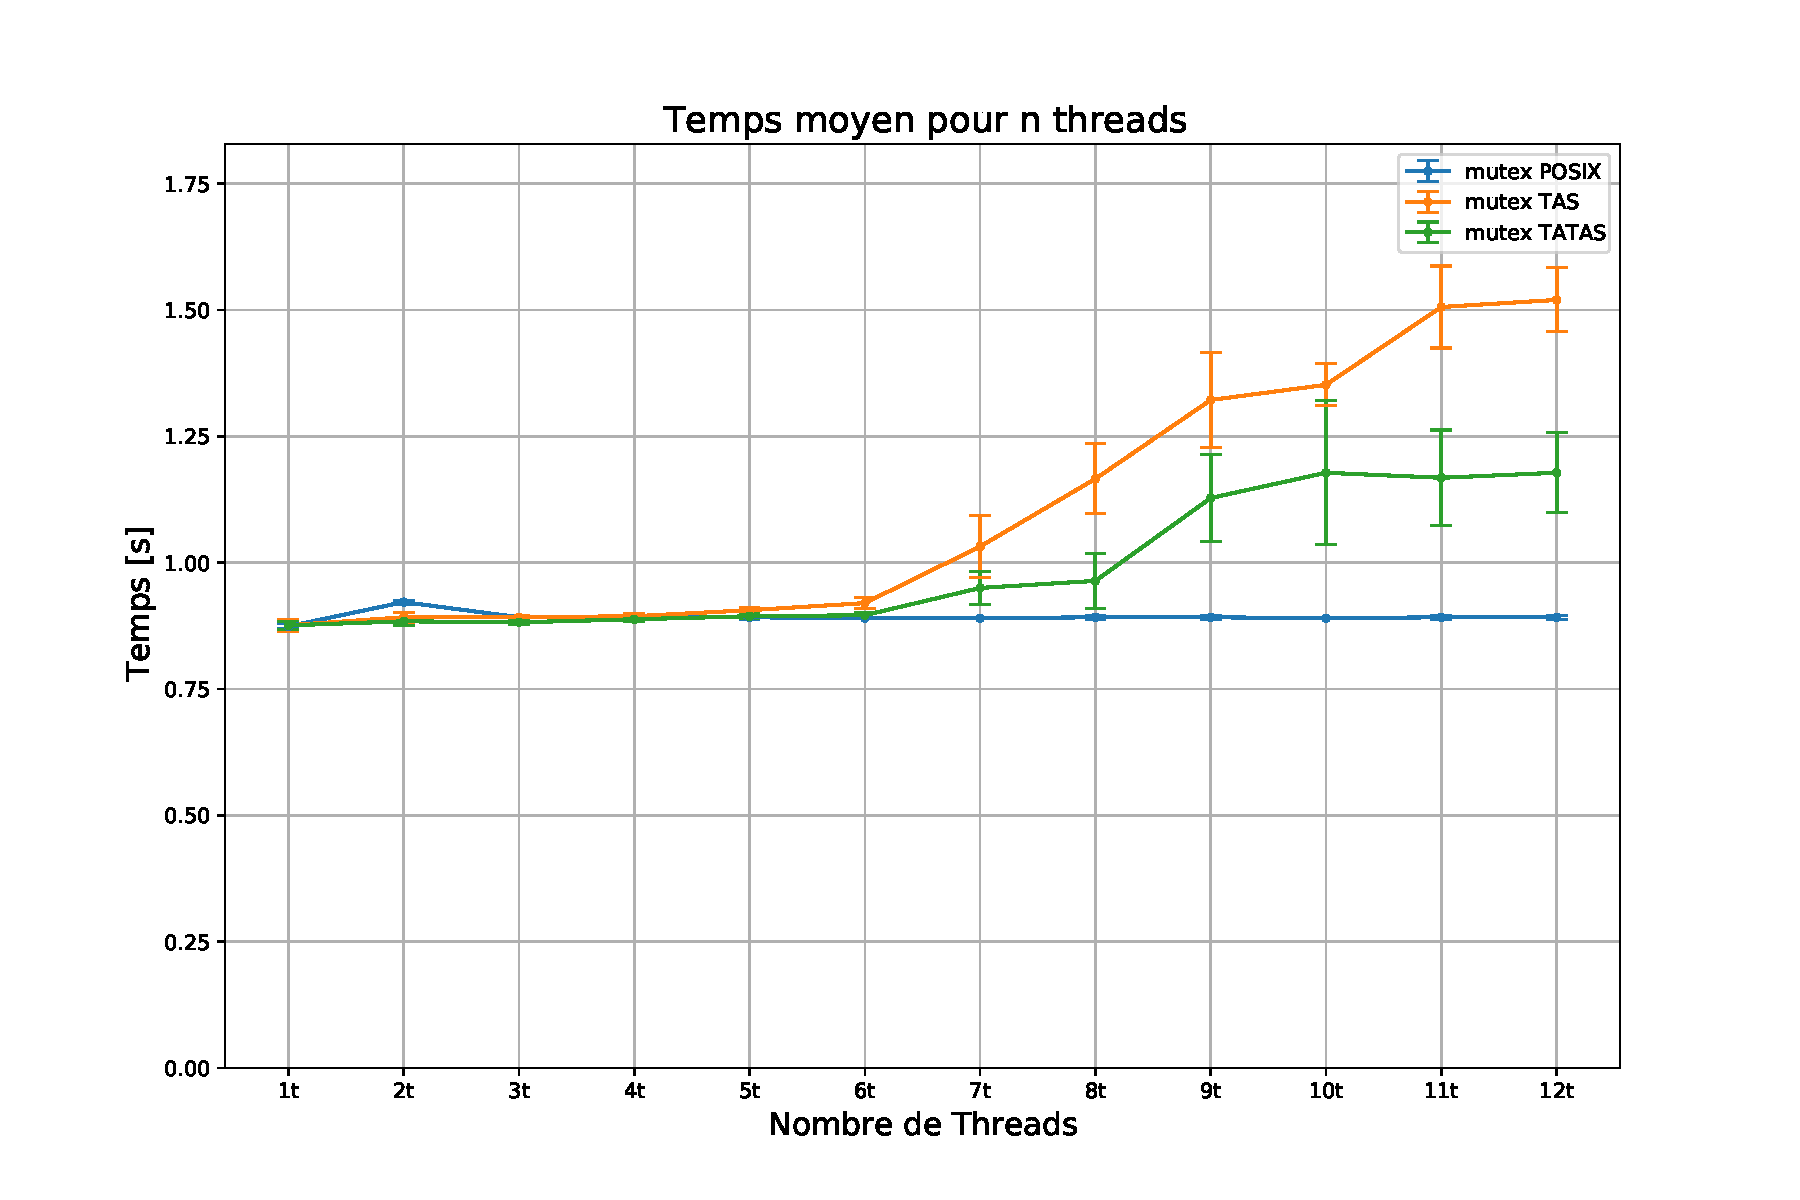
\includegraphics[scale=0.4]{img/spinlock.pdf}
    \caption{Temps d'exécution d'un verrou à attente active dans différentes conditions}
    \label{pic:spinlock}
\end{figure}

\noindent Nous pouvons observer que les performances des 3 types de mutex sont semblables et stables jusqu'au seuil de 6 threads, à partir duquel les performances divergent.
On peut ensuite observer que les performances de l'algorithme TAS se dégradent plus vite que celles de l'algorithme TATAS lorsque l'on augmente le nombre de threads. 

\noindent La stabilité des performances jusqu'à 6 threads peut être expliquée par le fait qu'il n'est pas nécessaire d'effectuer de changements de contexte pour terminer l'algorithme. 
A partir de 7 threads néanmoins, cela devient obligatoire et c'est cela qui va provoquer les dégradations de performances. Imaginons une situation avec 7 threads nommés de T1 à T7, supposons que les threads 1 à 6 possèdent un processeur et soient en mode Running. 
Supposons maintenant qu'après un certain laps de temps, le thread 2 unlock le mutex et termine son travail. Il sera donc nécéssaire d'effectuer les actions suivante pour pouvoir continuer l'exécution du programme : 
\begin{itemize}
    \item Déposséder le thread 2 de son processeur
    \item Effectuer un changement de contexte pour permettre à T7 d'effectuer son travail
    \item Un thread du processus entre dans sa SC et lock le mutex. 
\end{itemize}
On va donc avoir une forte contention sur le mutex lors de la libération de celui-ci, engendrant dans ce cas-ci 5 opérations ``xchg`` dont une seule sera fructueuse.\footnote{les threads 1,3,4,5,6 essayent d'acquérir le mutex et le 7 effectue son changement de contexte}
Le problème étant qu'un changement de contexte doit restaurer les variables globales du thread, ce qui est impossible durant l'exécution d'une opération \texttt{xchg} car le bus de cache est temporairement arrêté. 
Les changements de contextes de cette application avec plus de 6 threads seront donc très lents. La stabilité des mutex POSIX permet également de ne pas rejeter cette hypothèse. En effet nous savons que les mutex POSIX sont implémentés avec l'aide du noyau, 
plaçant les threads en mode Blocked lorsque ceux-ci tentent d'acquérir un mutex déjà acquit et les remettant en mode Ready lorsque le mutex se libère. Les mutex POSIX engendrent de nombreux changements de contextes, mais ceux-ci n'ont pas lieu lors de pic d'utilisation de l'instruction \texttt{xchg}.

\noindent Au vu des meilleures performances des mutex TATAS, j'ai choisi d'implémenter les sémaphores sur base de ceux-ci.
\section{Problème des philosophes}

\begin{figure}[h!]
    \centering
    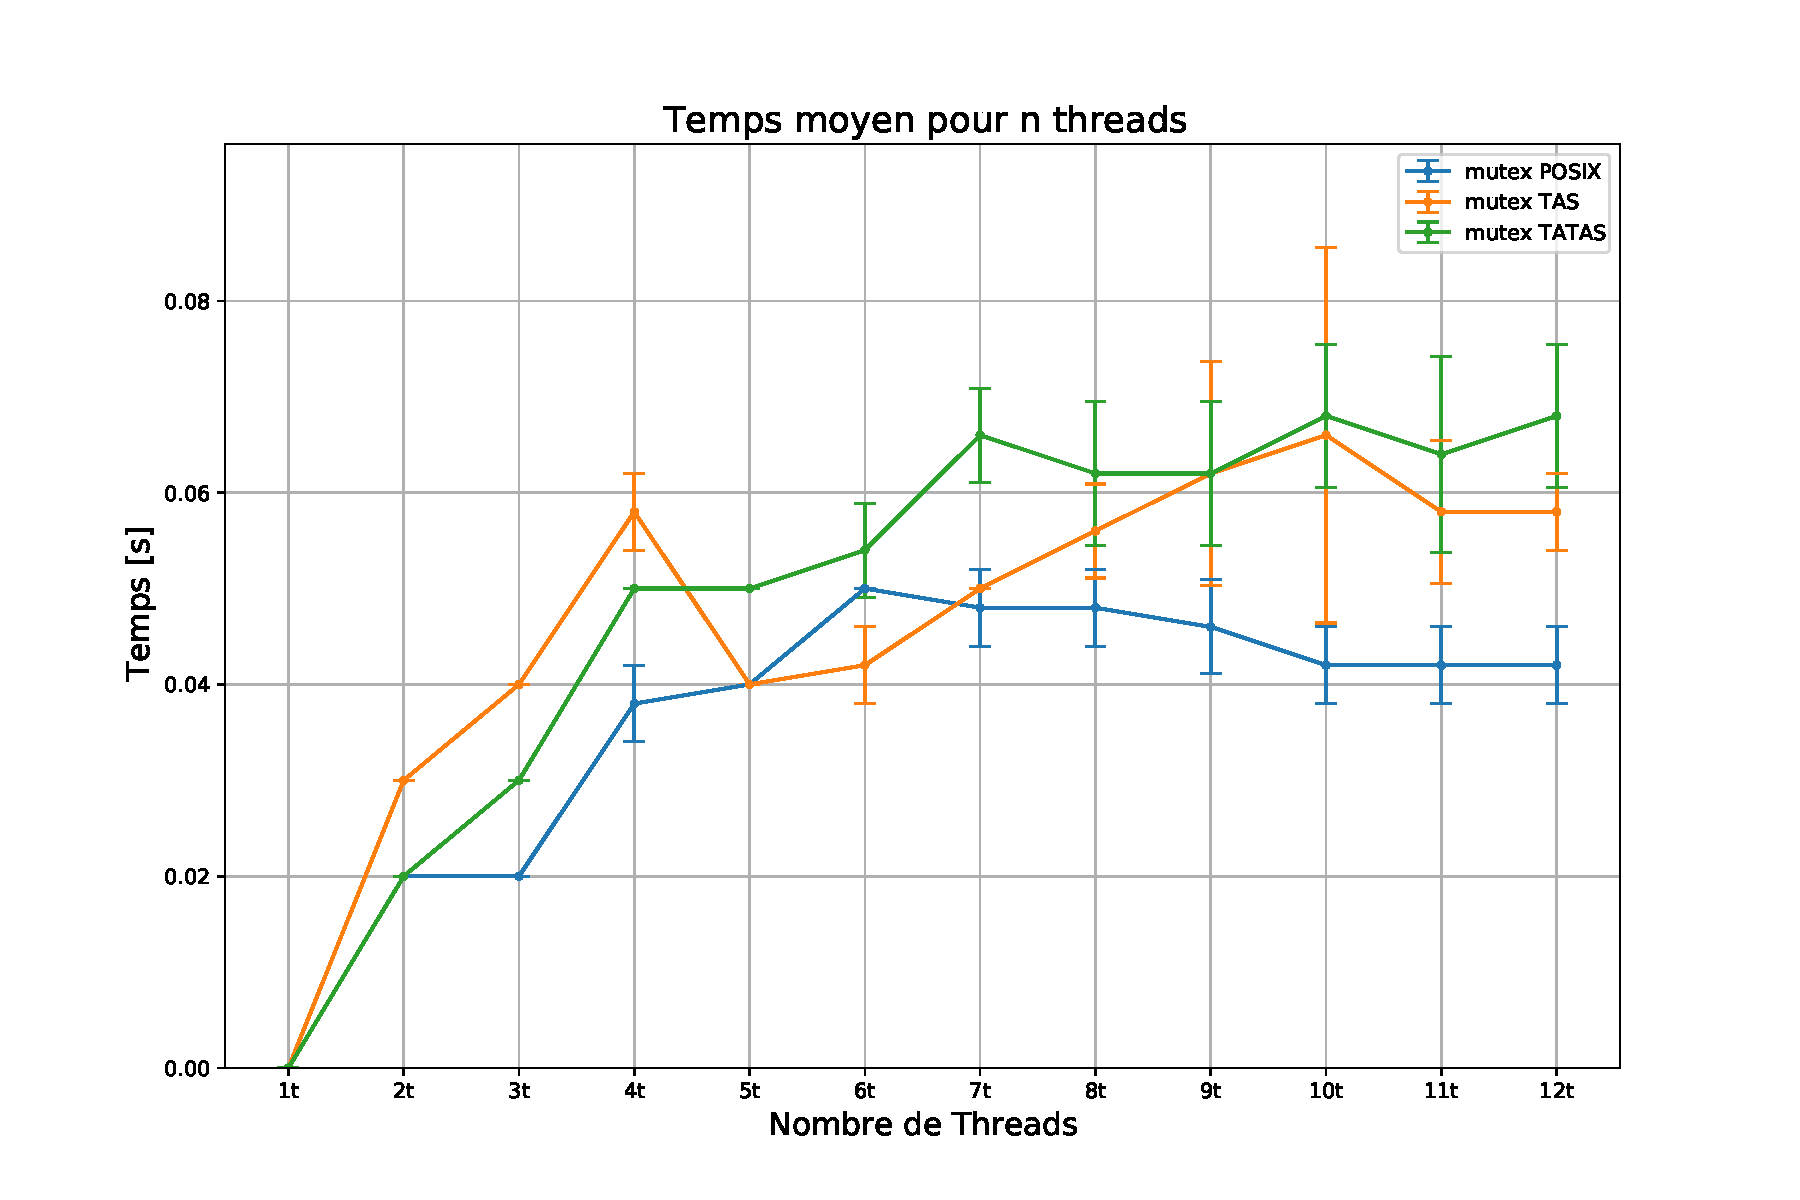
\includegraphics[scale=0.4]{img/philosophes.pdf}
    \caption{Temps d'exécution du problème des philosophes dans différentes conditions}
    \label{pic:philo}
\end{figure}

\noindent On observe que les deux courbes commencent par une phase de croissance pour se terminer par une phase de stabilisation.
On observe également que les mutex POSIX sont généralement plus stable que les spinlock TATAS. En effet on voit clairement que l'écart-type est bien inférieur. \\

\noindent Nous savons que théoriquement, le temps d'exécution est censé être constant. Suivant la parité du nombre de philosophes et en considérant la disposition des baguettes nous avons que si le nombre de philosophes est pair, la moitié des philosophes peuvent effectuer leurs opération pour ensuite laisser place à la seconde moitié, donnant un temps d'exécution constant.
Dans le cas où le nombre de philosophes est impair, $\frac{n-1}{2}$ philosophes peuvent effectuer leurs opérations en même temps, résultant également en un temps constant (théoriquement plus long que pour un nombre pair). \\

\noindent Mais nous n'observont pas du tout un temps d'exécution constant. Il y a donc une perte de performance dûe à la synchronisation. 
De plus, les spinlocks sont moins performant que les mutex POSIX pour cette application. Cela est cohérent avec ce que l'on a vu au cours : l'attente active est moins efficace lorsque le temps d'exécution d'une section critique (SC) est du même ordre de grandeur que le temps entre 2 accès à la SC.

\section{Problème des Producteurs-Consommateurs}

\begin{figure}[h!]
    \centering
    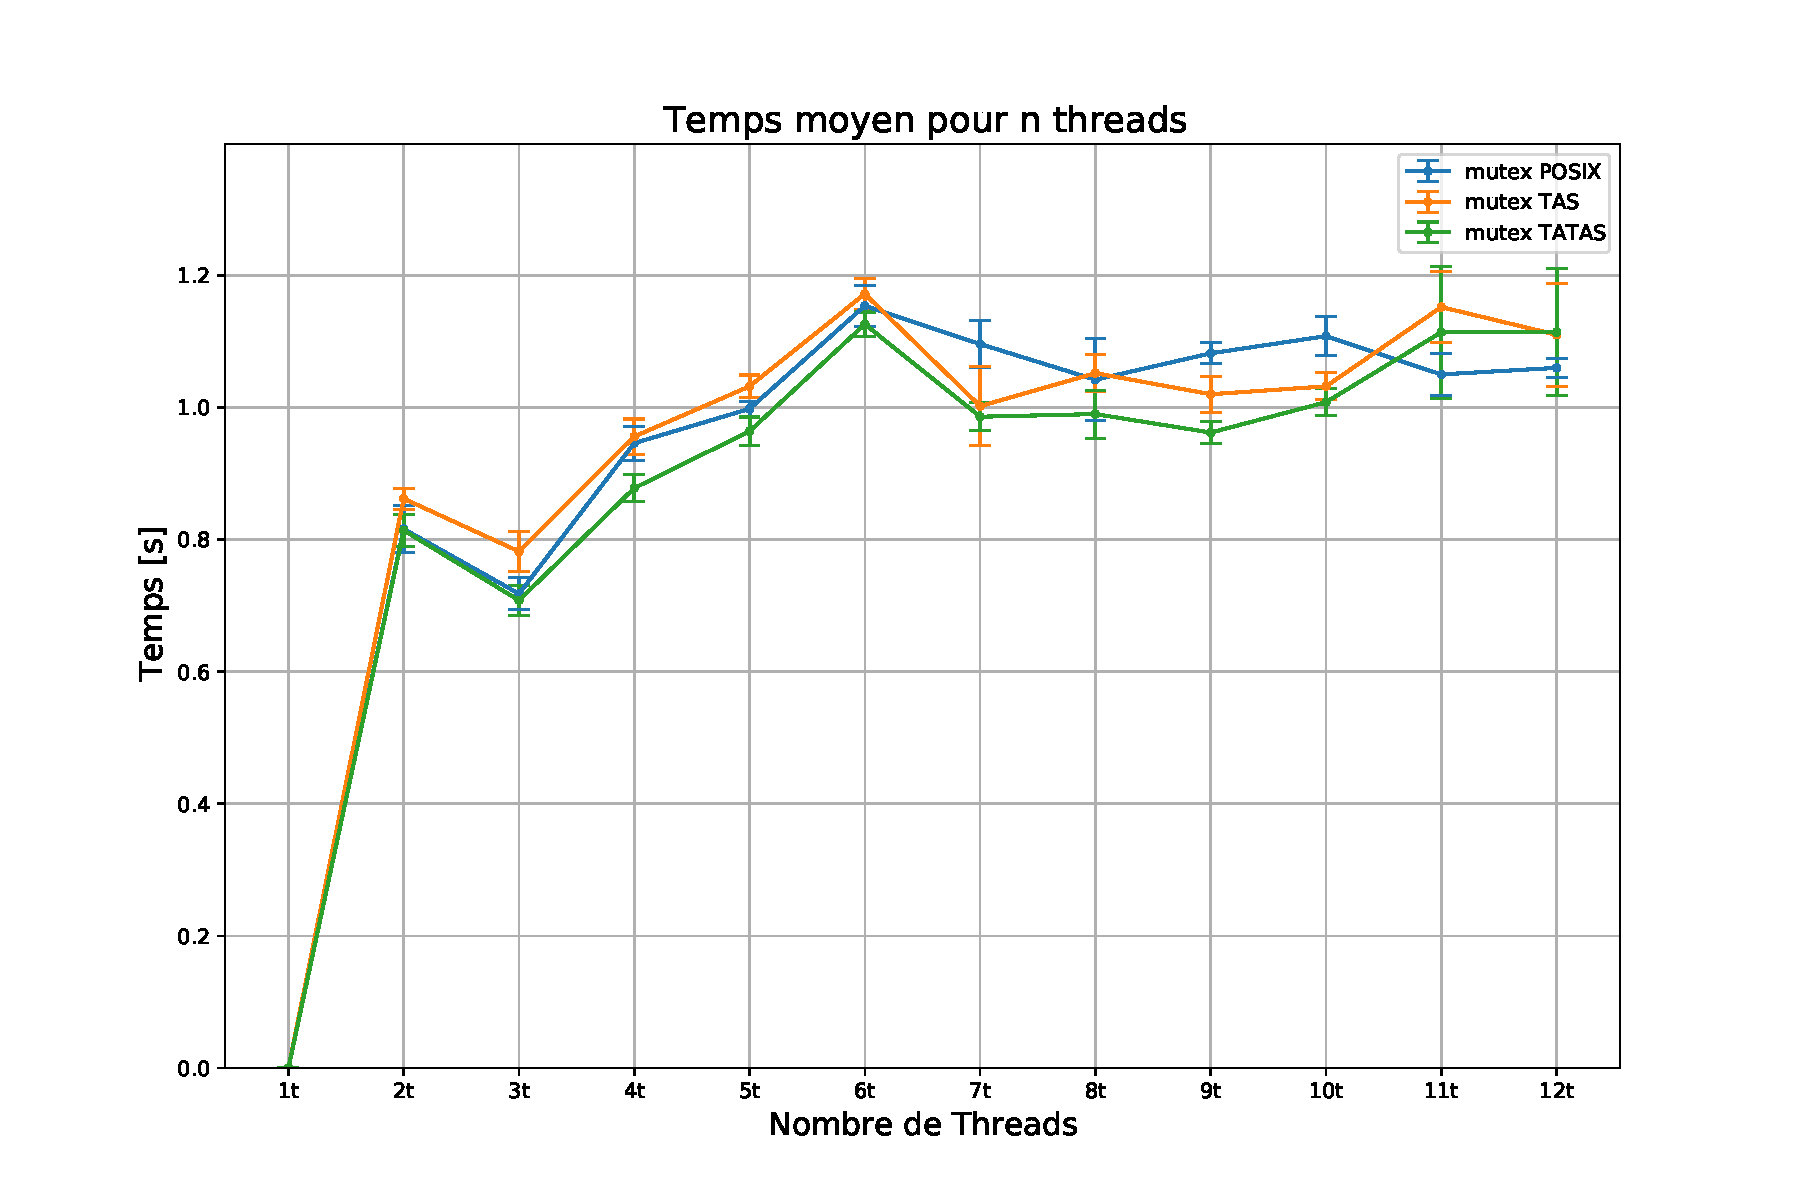
\includegraphics[scale=0.45]{img/prodcons.pdf}
    \caption{Temps d'exécution du problème des producteurs-consommateurs dans différentes conditions}
    \label{pic:prodcons}
\end{figure}

\noindent On peut remarquer ici que la différence de temps d'exécution entre les deux algorithmes est moins marquée que pour le problème des philosophes. Cela est dû au fait que 
le temps d'exécution des SC est ici négligeable par rapport au temps d'accès entre 2 SC. 
On remarque également que pour un travail équivalent le temps d'exécution augmente, il y a donc également une perte de performance dûe à la synchronisation.

\section{Problème des lecteurs-écrivains}

\begin{figure}[h!]
    \centering
    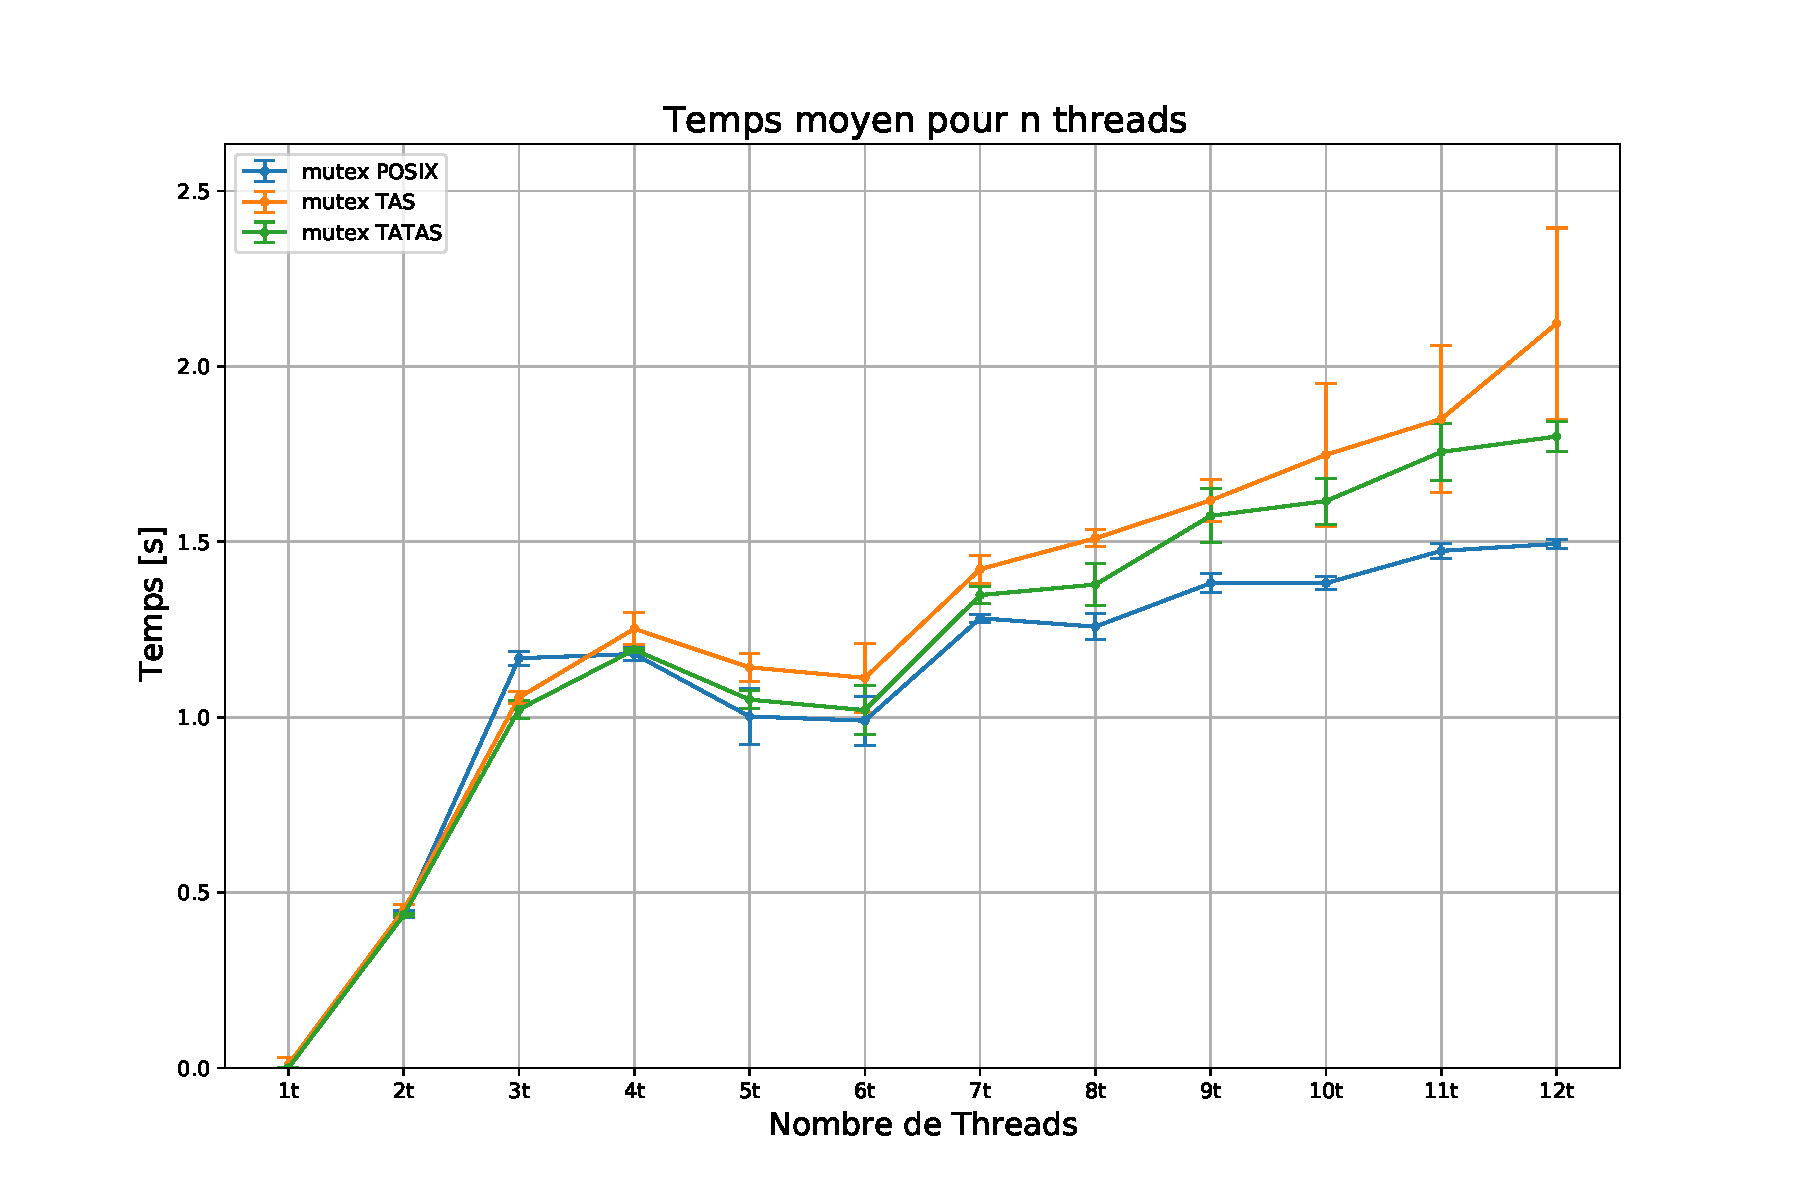
\includegraphics[scale=0.45]{img/readwrt.pdf}
    \caption{Temps d'exécution du problème des lecteurs-écrivains dans différentes conditions}
    \label{pic:readwrt}
\end{figure}

\noindent On observe que la tendance est généralement croissante pour les deux courbes, à l'exception d'une baisse au niveau des threads 5 et 6. On remarque également une divergence des deux courbes pour un nombre de threads supérieur à 7.
La divergence peut être expliquée de la même manière que celle dans le cas du problème des philosophes, à savoir que le temps d'accès entre 2 SC est négligeable par rapport au temps d'exécution des SC. 

\newpage
\section{Conclusion}

D'un point de vue théorique, j'ai pu apprendre lors de ce projet qu'ajouter des threads n'est pas synonyme d'amélioration de performances.
En effet, j'ai pu voir qu'il est nécessaire de prendre en compte le temps d'exécution des sections critiques ainsi que le temps entre 2 accès à celles-ci. 
J'ai également pu apprendre à effectuer des instructions atomiques en assembleur, tout en prenant conscience de l'impact de ces instructions sur les performances \textit{générales} de l'ordinateur. 
L'écriture d'opération en assembleur m'a également permis d'en apprendre davantage sur la gestion des registres des processeurs et les interactions de ces derniers avec le bus de cache. \\

\noindent D'un point de vue pratique, je me suis forcé à écrire du code propre et \textit{générique}. Ce qui m'a permit de découvrir l'utilité des unions afin d'écrire des interfaces facilement utilisables avec des types de données différentes. \\

\noindent En conclusion, ce projet m'a permit d'ouvrir les yeux sur le point de vue \textit{hardware} du multithreading tout en améliorant mes capacités d'écriture et d'analyse de code nécéssaire à tout programmeur.


\end{document}

